%!TEX TS-program = xelatex
%!TEX encoding = UTF-8 Unicode

\documentclass{../Dissertate}
%% \documentclass{../DissertatePrint}
%% \usepackage{comment}
%% \excludecomment{figure}
%% \let\endfigure\relax

\begin{document}

\doublespacing

\setcounter{chapter}{5}
\chapter{Intuition vs. Reflection in Reasoning}

\section{Introduction}

In Chapter 1, I discussed how people can
draw on different sources of information in induction.
In this chapter, I report a pair of experiments in which
two such sources --- perceptual similarity,
and conceptual knowledge in the form of category membership ---
are placed into conflict.
This was done using a mouse tracking version of
\citegap{Gelman1986}{'s} inductive triad task.
In Experiment 1, participants learned a biological property of
different species in the natural world, and were asked to
project each property to one of two species,
one of which belonged to the same taxonomic group as the base species.
In the conflict condition, but not the control condition,
the base and the foil species looked alike,
and so perceptual cues conflicted with conceptual knowledge.
In Experiment 2, participants completed a similar task,
but using artificial categories, learned at the start of the experiment.
I also manipulated the nature of the properties
participants reasoned about in Experiment 2, between participants,
to reveal how this modulated participants' inferences.

As discussed in Chapter 1,
theories of inductive reasoning can be organised into two groups.
One class of theory relies on conceptual knowledge
about the categories to which different entities belong,
and the relations between these categories.
Category membership is perhaps the most fundamental 
such form of conceptual knowledge that we can use as the basis for induction.
According to contemporary accounts of categorisation
\citep[see][]{Murphy2004,Rosch1988},
a category consists of a set of entities that have attributes in common.
Therefore, if we know the category to which something belongs,
we may believe that it has attributes
that we know are found in other members of that category
\citep{Murphy2004,Osherson1990}.
That adults can reason in this way has never been in question,
and indeed this idea is central to the very notion of categorisation
\citep{Mill1856,Gelman1986}.
This principle applies equally to inferences about people,
where it is better known as \emph{stereotyping}
\citep{Greenwald1995,Oakes1994}.
% The evidence that we do use knowledge about categories when reasoning
% is considerable, and indeed this should be self-evident,
% and so will not be reviewed in detail here.
% Few results in literature on inductive reasoning in adults
% \citep[see][for reviews]{Feeney2007,Hayes2010}, for example,
% can be accounted for without recourse to category-based inference.
Strikingly, people rely on categorical information
even when it is disadvantageous to do so.
Murphy and Ross \citep{Murphy2012,Murphy2010,Malt1995,Murphy1994}
showed, for instance, that when it is not certain
to which category an entity belongs,
participants nevertheless reason on the basis
of it belonging to the most likely category.
\citet{Mishra2010} also report a \emph{border bias} phenomena:
distant locations in the same state (for instance New York City, and Buffalo, New York) 
are perceived as physically closer, and more likely to share properties,
than closer locations divided by state lines (New York City and Princeton, New Jersey.

% \aside{I could also talk about language, and developmental trends here,
%   but I don't think I will}
Category membership is also at the core of many more sophisticated theories of induction
\citep[i.e.][]{Osherson1990,Griffiths2009,Kemp2009},
which combine information about category membership
with knowledge about the relationships between various categories.

% Similarity
Other theories of induction are not based on category membership.
Similarity between entities is the most common kind of
non-categorical information proposed to underlie induction:
entities that are similar (i.e. that share many features)
are more likely to also share a new feature
than things that are dissimilar.
This principle forms the basis of many feature-based accounts of induction
\citep{Sloman1993,Rogers2004,Sloutsky2004,Fisher2015},
discussed in Chapter 1.
\citet{Fisher2015} draw a distinction between two kinds of similarity,
based on either overlapping perceptual cues,
or on shared features in our mental representations.
With regard to adults' inferences,
the focus has been on the latter, \emph{representational} similarity.
While it is usually assumed that adults
are not swayed by inappropriate perceptual cues,
overlapping features in our mental representations of entities
form the basis of both \citegap{Sloman1993}{'s} Feature Based Induction model,
and \citegap{Rogers2004}{'s} Semantic Cognition accounts of induction.
\citet{Sloutsky2008,Sloutsky2004} propose
an analogous model to explain children's inferences,
based on perceptual similarity.
%% Interestingly, in contrast to findings \citep[i.e.][]{Murphy2012} that
%% reasoning under uncertainty is based on the most likely categorisation only,
%% inferences made under speeded conditions \citep{Chen2013,Verde2005,Newell2010}
%% are usually made on the basis of shared properties,
%% rather than category membership.

Given the importance of conceptual knowledge such as category membership in induction,
why then might perceptual similarity play a role?
One reason is that similarity is a useful proxy for shared category membership:
categories are collections of things that share properties, 
including visible features,
and things which look alike tend to belong to the same category.
Furthermore, regardless of category membership,
attributes tend to be correlated in the real world:
things that share properties we know of
are more likely to also share novel properties
\cite[see, e.g.,][]{Kemp2012}.
For both of these reasons, under many circumstances 
similarity --- even perceptual similarity ---
and conceptual knowledge will support the same inferences.
However, there do exist problems for which
these two kinds of information disagree,
most notably when reasoning about entities
that look more like members of a different category
than members of the category to which they belong
(that is, visually \emph{atypical} category members).
The archetypal examples of such atypical entities are whales,
which are mammals, but bear closer resemblance to fish
than to other mammals.


% Development
This chapter, like the rest of this thesis, focuses on adults' reasoning.
However, there has been little prior research on the role of
simple perceptual cues in adults' inductive reasoning,
perhaps because it would appear self-evident that
adults rely on conceptual knowledge,
or at least representational similarity.
There has been extensive debate, however,
as to whether young children make use of conceptual knowledge at all,
or if their inferences are simply driven by perceptual similarity.

There are a number of reasons to believe that children may rely on perceptual-cues,
rather than conceptual knowledge, in induction.
Conceptual knowledge must be acquired through instruction and experience,
and so early inferences, by which infants and children make sense of the world,
must be driven by a simpler, associative process like visual similarity
\citep{Westermann2013,French2004}.
In recent years, it has also become apparent that
simple associative mechanisms can produce
inferences that are surprisingly complex and flexible \citep{Sloutsky2008,Hinton2014}.
Indeed, \emph{deep neural networks} ---
neural networks, using simple associative principles but with many layers ---
are at the forefront of modern machine learning and artificial intelligence research
\citep{Mnih2013,Hinton2006}.

Sloutsky \citep[i.e.][see \citealp{Sloutsky2003,Sloutsky2010} for reviews]{
  Sloutsky2008,Sloutsky2007,Sloutsky2004a}
has therefore argued that young children's reasoning
is often based on such perceptual cues,
with reliance on conceptual knowledge arising later in development.
In contrast, Gelman 
\citep[i.e.][see \citealp{Gelman2011a,Gelman2004a} for reviews]{
  Gelman2013c,Rhodes2009,Gelman2007a,Gelman1986}
argues that even toddlers
 % \aside{Or younger?}
rely on conceptual knowledge about the world,
and naive theories \citep{Gopnik2003,Carey2009} 
to make inferences about the world around them.

\citegap{Gelman1986}{'s} triad task,
discussed in Chapter 1,
has been widely used as a testing ground
for these competing accounts.
Recall that in this task,
children were presented with images of two entities
(a flamingo and a bat, for instance),
given their labels (``bird'' and ``bat''),
and told a property of each
(``This bird's legs get cold at night'';
``This bat's legs stay warm at night'').
They were also shown a third species
(a blackbird in this example, labelled ``bird'',
but which more closely resembled the bat)
and asked to indicate which property it would have
(``Do this bird's legs get cold at night, like this bird's,
or stay warm at night, like this bat's?'').
\citet{Gelman1986} report that children as young as four
predominantly resist the perceptual cue,
and reason based on shared category membership --
projecting a property from the flamingo to the blackbird,
in this case.
On the other hand, \citet{Sloutsky2007} present results with artificial categories
that seem to show children ignoring category membership
in favour of perceptual similarity.
\citet{Gelman2013c}, however, demonstrate that
this result only holds under certain circumstances,
specifically, when the nature of the learned categories is obscure
and not obviously relevant to the properties being projected
(i.e. a creature's ratio of buttons to fingers).

% Hybrid theory
In Chapter 1, I introduced \citegap{Bright2014a}{'s} hybrid theory of induction.
This proposes that when reasoning inductively,
we can draw on either simple, associative knowledge --- such as similarity ---
or structured knowledge about the relationships between
entities and the categories they belong to.
The distinction in question in the current chapter,
between perceptual cues and simple conceptual knowledge,
is perhaps a more fundamental one than that made by
\citet{Bright2014a} between associative and structured knowledge.
Nevertheless, their hybrid account could easily
be extended to include it.

A prediction that emerges from this extended version of the hybrid theory
is that even adults' inferences may be influenced by perceptual similarity.
To date, there has been little evidence
suggesting that adults' inferences are driven by perceptual cues.
However, as discussed in Chapter 1,
this may in part be because methods used in previous work
were poorly suited to revealing such conflict,
and so in this chapter I explore this question
using the mouse tracking paradigm.
However, previous studies using this triad task
\citep[i.e.][]{Gelman1986,Sloutsky2007,Gelman2013c}
both with adult and child participants,
have only included trials in which perceptual similarity
and conceptual knowledge have conflicted.
Typically, adults overwhelmingly respond on the basis
of conceptual knowledge on such trials,
while the debate has focused on whether children's responses
are driven by conceptual knowledge \citep{Gelman1986,Gelman2013c}
or perceptual similarity \citep{Sloutsky2007}.
By not including trials in which both cues agree, however,
these experiments do not make it possible to see
if adults' reasoning was influenced by perceptual cues
in addition to conceptual knowledge:
when perceptual cues disagree with conceptual knowledge,
participants may be less likely to give the conceptually-cued response,
or slower to do so, or be otherwise conflicted,
than when the cues agree.

Therefore, in this chapter, I present two experiments, with adult participants,
in which perceptual cues either conflict or agree with conceptual knowledge.
If adult induction is in part driven by perceptual cues,
participants should be less likely to generalise
from a base entity to a conceptually-related one
when the alternative, foil entity is visually similar to the base.
Recording participants' mouse cursor trajectories,
it is also possible to investigate how these kinds of information interact over time.
If participants are driven by \emph{either} perceptual similarity
\emph{or} conceptual knowledge on each trial,
they should move the mouse directly to one or other response.
Alternatively, if participants are initially driven by
quickly-available perceptual cues,
but draw on conceptual knowledge later in the reasoning process,
we may see reversal trajectories, as participants
initially move towards the perceptually-cued option,
and change direction mid-trial.





\section{Method}

\subsection{Participants}

One hundred and thirty one students at Queen’s University Belfast
participated in exchange for course credit.

\subsection{Materials}

Eight problems were adapted from
\citegap{Primi2015}{'s} extended version of the CRT.
Each of these problems was modified to create a set of
eight corresponding non-conflict problems,
in which the intuitively appealing responses were also the correct ones
(see the Appendix~\ref{appendix:exp6_stimuli}).
Participants were randomly allocated to complete either
conflict versions of items 1, 3, 5, and 7
and no-conflict versions of the rest, or vice versa.
Each problem was presented in a 4-option multiple choice format.
For the conflict items, the possible responses were the correct option,
the incorrect heuristic option, and two incorrect foil options.
For the non-conflict items the correct intuitive option was presented
with three incorrect foils.

\subsection{Procedure}

The experiment was administered on personal computers,
programmed using PsychScript (see Chapter 2),
and run in the web browser.
Participants were instructed to respond in their own time to each CRT problem
by clicking on one of the four response options
presented in the four corners of the display
(Figure~\ref{fig:exp6-screenshot}).
Participants were not made aware of
the mouse tracking aspect of the experiment in advance. 

\begin{figure}[ht]
  \centering
  \includegraphics[width=\figurewidth]{imgs/exp6-screenshot.png}
  \caption[A screen shot from the CRT, Experiment 6.]{
    \label{fig:exp6-screenshot}
    A screen shot from the CRT.
  }
\end{figure}

Each problem was preceded by onscreen instructions to
click on a button marked ``Go'', presented in the centre of the monitor.
This was done to ensure the mouse cursor was located
in the same central position at the beginning of each trial.
The button was then replaced by the problem text
and the four response options appeared simultaneously in the corners
(Figure~\ref{fig:exp6-screenshot}).
The response options were randomly assigned to the four locations on each trial,
with the constraint that the correct and heuristic response options
were always adjacent for conflict problems.
The mouse cursor was no longer visible at the onset of each trial
to prevent it from obscuring the question text.
The cursor reappeared once it had been moved more than 5\% of the width of the display.
Mouse cursor location was recorded every 20 msec.


\section{Results}

The current results section follows the same
format used previously in this thesis;
I first present analyses of participants' responses,
followed by measures of conflict on trials where a particular response was given,
then the cursor transition probabilities,
and finally the time course data.
Each of these analyses is broken into three sections.
First, I investigated what happens on trials where both cues conflict.
Then, I tested the effect of descriptions on base rate-driven reasoning.

There were three kinds of trial in which
participants could use base rate information in this task:
trials where both the base rate and the description cued the same response
(i.e. the description agreed with the base rate),
trials where the base rate provided the only useful information
(the description was uninformative),
and trials where the description cued the opposite response
(the description disagreed with the base rate).
Most dual process theories would predict that descriptions,
being more easily and readily processed,
should interfere with base rate-based reasoning.

I also test the effect of base rates on description-cued reasoning.
There were also three types of trial where
participants could rely on the description:
trials where the description and the base rate cued the same response
(i.e. the base rate agreed with the description)
trials where only the description was useful
(the base rate was uninformative; 500:500),
and trials where the base rate cued the opposite response
(the base rate disagreed with the description).

Analyses were conducted using multilevel models,
with random intercepts for each participant, and for each problem,
unless otherwise stated.
As before, log-linear models were used for the latency data
(reading time, movement initiation time, and response time),
and logistic models for analysis of participants' responses,
and the transition probability analysis.

\subsection{Responses}

Table~\ref{tab:exp5_responses} shows the proportion of responses
consistent with each cue in each condition.
When the cues disagreed, participants selected
the description-cued response on 80.4\% of trials,
and the base rate-cued response on 19.6\%,
a statistically significant difference (z = 5.958, p < .0001).


\begin{table}[h]
  \centering
  \caption[Participants' responses, Experiment 5.]{
    Responses consistent with each cue, according to whether the
    other cue agreed with it, is uninformative, or disagreed with it, in Experiment 5.
    \label{tab:exp5_responses}
  }
  \begin{tabular}{l R{2.5cm} l l R{2.5cm}}
    \toprule
    Description   & Base rate responses & & Base rate     & Description responses\\
    \cline{1-2}
    \cline{4-5}
    Agreed        & 94.4\%              & & Agreed        & 94.4\%\\
    Uninformative & 69.4\%              & & Uninformative & 93.6\%\\
    Disagreed     & 19.6\%              & & Disagreed     & 80.4\%\\
    \bottomrule
  \end{tabular}
\end{table}

\subsubsection{Effect of descriptions on base rate choices}


Descriptions had a significant main effect on
the probability of participants' giving the base rate-cued response
($\chi^2$ = 741.6, DF = 2%
\footnote{
  Recall from Chapter 2 that Chi-squared tests
  are used in place of ANOVA F tests
  for mixed models analysis ---
  a significant chi-squared test denotes
  a significant main effect of condition here.
  }, p < .0001).
Participants were significantly more likely\footnotemark
to give the base rate cued response when
the base rate and description agreed (94.4\% of trials)
than when the description was uninformative (69.4\%)
or when the description disagreed with the base rate (19.6\%)
They were also significantly more likely to do so
when the description was uninformative
than when the description disagreed
(z's > 8, p's < .0001).

\footnotetext{All post-hoc comparisons report
  Tukey adjusted p values and confidence intervals.}

Figure~\ref{fig:exp5_br_acc} plots the number of 
base rate cued responses given by each participant, by condition,
and indicates that these effects seem to be operate consistently
across all participants, rather than being driven
by a subset of participants who are influenced by the description.
Of the 50 participants, 49 were less likely 
to give the base rate cued response
when base rates and descriptions disagreed than when they agreed,
and 1 always gave the base rate cued response.

\begin{figure}[ht]
  \centering
  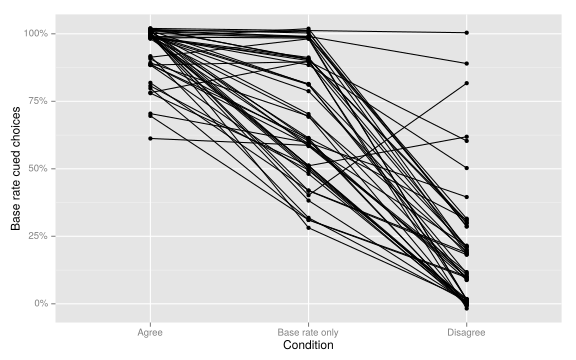
\includegraphics[width=.6\textwidth]{imgs/exp5_br_acc.pdf}
  \caption[Individual differences in the effect of descriptions
  on participants' responses, Experiment 5.]{
    Number of base rate responses per condition, by participant, in Experiment 5.
    \label{fig:exp5_br_acc} }
\end{figure}

\subsubsection{Effect of base rates on description choices}


Base rates had a significant main effect on
the number of description-cued responses given
($\chi^2$  = 67.7, DF = 2, p < .0001).
Pairwise comparisons showed that participants were
less likely to give the description-cued response
when the base rate disagreed with the description (80.4\%)
than when it agreed (94.4\%;
$e^{\beta}$ = 0.20, CI = [0.12, 0.36], z = 6.655, p < .0001)
or when the base rate was uninformative (93.6\%;
$e^{\beta}$ = 0.24, CI = [0.14, 0.42], z = 6.128, p < .0001).
There was no difference between trials in which the base rate agreed
and those where the base rate was uninformative (z < .3, p > .7),
with both conditions close to ceiling.
Therefore, participants were at least in some way
sensitive to the base rate information, and in a minority of cases
relied on it instead of the description when the two conflicted.

Once again, it is useful to investigate individual differences in this effect.
The left panel of Figure~\ref{fig:exp5_description_acc} shows
the proportion of description-cued responses given by each participant by condition.
This shows three participants who were substantially less likely
to give the description-cued response when the base rate disagreed with it.
The right panel shows the difference, for each participant,
in the number of description-cued responses given
from when the base rate agreed to when it disagreed.
This shows that, along with the 
three participants who showed a substantial change,
most participants showed a moderate effect in the same direction:
they were slightly less likely to select
the description-cued response when the base rate disagreed with it,
suggesting that base rates had some effect on the majority of participants.
Out of 50 participants, 28 were less likely
to select the description-cued response when the base rate disagreed,
13 were equally likely to do so (including 10 who always gave this response),
and 9 were actually more likely to select the description-cued response
when the description disagreed.

\begin{figure}[ht]
  \centering
  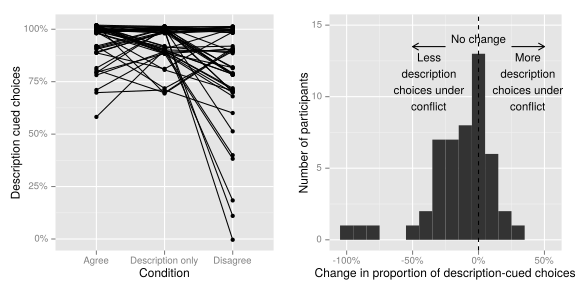
\includegraphics[width=\figurewidth]{imgs/exp5_description_acc.pdf}
  \caption[Individual differences in the effect of base rates
  on participants' responses, Experiment 5.]{
    \label{fig:exp5_description_acc}
    Left: Proportion of base rate-cued responses given in each condition,
    by participant.
    Right: Difference in the proportion of description-cued responses given
    by each participant between when the base rate agreed and disagreed with
    the description. Values below 0 indicate a participant was less likely
    to select the description-cued response when it conflicted with the base rate
    than when it agreed.
  }
\end{figure}


%%% Local Variables: ***

\subsection{Results}

\subsubsection{Post Test Check}

For each stimulus set used in the experiment,
participants correctly said that the base species
and the correct response species 
belonged to the same taxonomic group (accuracy > 70.5\%, p's < .01),
and that the moderate and strong foils
had the appropriate relationship (food chain or shared habitat)
with their base species (accuracy > 75\%, p's < .001).
Therefore, no data were excluded from the analyses on these criteria.
Full post-test results can be found in Appendix~\ref{appendix:exp4_posttest}.

\subsubsection{Reasoning Accuracy}

In order to analyse data from the reasoning trials,
for each trial I divided that participants' rating of
the association between the base and the correct species
by their rating of the association between the base and the foil.
This produced a ratio reflecting the extent to which
that participants' associative knowledge
favoured one or other response option.
Values of this ratio ranged from $\frac{1}{9}$
($.111$; association of 1 for the correct species, and 9 for the foil),
to $\frac{1}{1}$ (equal association for both species),
to $\frac{9}{1}$
(association of 9 for the correct species, and 1 for the foil).

For each analysis, I log-transformed this ratio
to create a normally-distributed linear predictor,
as is standard practice when using ratios as regression predictors \citep{Gelman2007}.
Note that $log(\frac{1}{1}) = 0$,
and correspondingly $log(\frac{>1}{1}) > 0$ and $log(\frac{1}{>1}) < 0$
(see Figure~\ref{fig:exp4_log_transform}).
Therefore, when using the log-transformed ratio as a predictor,
a positive regression weight means that
the dependent variable is greater/more likely when the ratio is greater than $\frac{1}{1}$,
or in other words, when the association rating favours the correct response.

\begin{figure}[h]
  \centering
  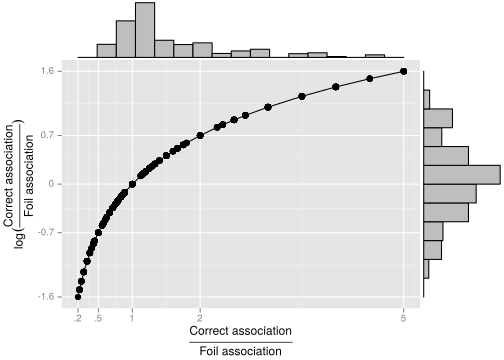
\includegraphics[width=.7\textwidth]{imgs/exp4_log_transform.pdf}
  \caption[The log-transformed association ratio, used as a predictor in Experiment 4.]{
    To analyse data from Experiment 4,
    each participants' rating for the association between
    the base species and the correct response species
    was divided by their rating for
    the base and the foil species, to form an association ratio.
    These ratios were log-transformed to use as predictors in regression analyses:
    after log-transformation, the difference between 1 and 0.2 (dividing by five)
    is the same as the difference between 1 and 5 (multiplying by five).
    \label{fig:exp4_log_transform}
  }
\end{figure}

Some aspects of the analyses based on this ratio are slightly unusual,
and so I will go through my first analysis,
predicting participants' responses,
in detail to familiarise readers with the method.
Figure~\ref{fig:exp4_ratio_accuracy} plots the proportion of correct responses 
(choosing the species belonging to the same taxonomic group as the base) given, on the y axis,
as a function of the association ratio, on the x axis.
Note that the x axis is log-scaled.
For plotting, I have divided the log-transformed ratio into 13 equal bins,
and plotted the mean and standard error of the dependent variable within each bin.
For the analyses, I fit log-linear, or logistic mixed models,
with random intercepts for each participant, and for each stimulus set.
The log-transformed association ratio from each trial was used as the predictor in the models.

\begin{figure}[h]
  \centering
  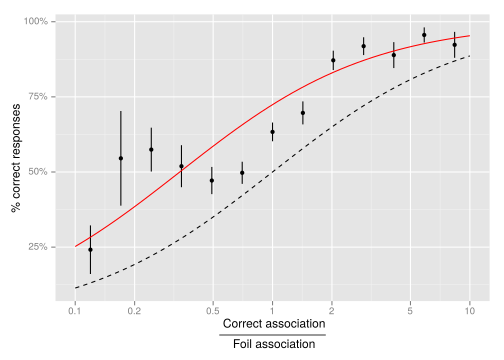
\includegraphics[width=.6\textwidth]{imgs/exp4_ratio_accuracy.pdf}
  \caption[Effect of the association ratio of participants' accuracy, Experiment 4.]{
    Correct responses on Experiment 4, as a function of
    the association ratio in favour of the correct species.
    As the ratio increased in favour of the correct species,
    participants became more likely to select that species.
    The fitted model (red line) included a significant positive intercept term,
    meaning that participants were more likely to select the correct species
    than would be predicted based on the association ratio alone (dashed black line).
    \label{fig:exp4_ratio_accuracy}
  }
\end{figure}

The association ratio was a significant predictor of the odds of a correct response
($\beta$ = 0.89, CI = [0.68, 1.1], z = 8.604, p < .0001).
Interpretation of the regression $\beta$ here is not straightforward,
but positive $\beta$s indicate that the dependent variable
(odds of a correct response) was positively related to
the size of the association ratio in favour of the correct response.
Fortunately, we can simply look to the predicted values from this model
(solid red line in Figure~\ref{fig:exp4_ratio_accuracy})
to see the magnitude of this effect.

An unusual property of these models is that
the intercept parameter is also meaningful.
As the log-transformed association ratio is the only predictor in the model,
the intercept reflects the expected value
when this predictor is at 0, or in other words, for a ratio of $\frac{1}{1}$.
If participants do not make use of structured knowledge,
we would expect participants to select the correct species
50\% of the time for such trials, something that would correspond to an intercept of 0.
The dashed black line in Figure~\ref{fig:exp4_ratio_accuracy}
shows the predicted values for such a model, with intercept 0.
A significant positive intercept means that
participants were more likely to select the correct species
than would be expected from the association ratio alone,
while a negative intercept means they were less likely.
There was a significant positive intercept term in this model
($logit(\beta)$ = 72\%, CI = [56\%, 85\%], z = 2.585, p = .0010).
I report the $logit$ of the regression $\beta$ weights here
as an easily interpretable measure of how much participants
were biased towards the correct species.
In this case, $logit(\beta)$ reflects how often
participants would be expected to select the correct species
on trials where the association ratio = $\frac{1}{1}$,
according to the fitted model
(i.e. where the red line on Figure~\ref{fig:exp4_ratio_accuracy}
crosses $1$ on the x axis).
Together, these results mean that participants were
a) more likely to select the correct species when
they rated it as being more strongly associated with the base
than the foil was, and
b) biased towards the correct option rather than the foil
beyond the effect of the association ratio.

\begin{figure}[h]
  \centering
  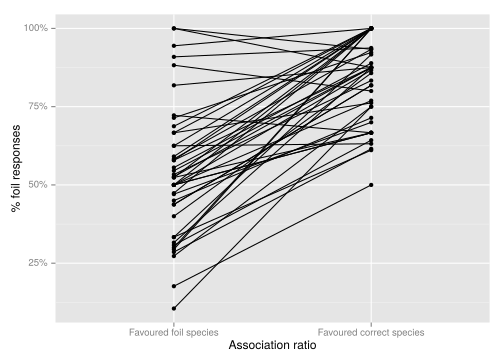
\includegraphics[width=.7\textwidth]{imgs/exp4_acc_ids.pdf}
  \caption[Proportion of correct responses
    given by each participant, by association ratio,
    in Experiment 4]{
    Participants' number of correct responses
    on trials where the association ratio favoured either
    the correct species or the foil species.
    40 of 44 participants were more likely to select the correct species
    when the association ratio favoured it
    than when the ratio favoured the foil.
    \label{fig:exp4_acc_ids} }
\end{figure}

To analyse individual differences in the number of correct responses
(Figure~\ref{fig:exp4_acc_ids}),
I calculated the number of correct responses given by each participant
both when the association ratio favoured the foil species,
and when it favoured the correct species,
excluding trials where species were rated as equally associated.
Of the 44 participants, 40 were more likely to select the correct species
when the association ratio favoured it,
and 4 were less likely to do so.
Therefore, it appears that almost all of my participants
were influenced by the association between species.

\FloatBarrier
\subsubsection{Correct Responses}

Analysing trials where the correct species was selected,
the association ratio had no effect on participants' movement initiation times
(mean = 574 msec, SD = 285; t(529.6) = 0.387, p > .6).
There was a marginally significant effect of the association ratio
on participants' response latencies
(mean RT = 1509, SD = 567;
$e^{\beta}$ = 98\%, CI = [96\%, 100.4\%], t(787.1) = 1.647, p =.100),
meaning that participants were marginally faster to respond correctly
as the association ratio in favour of the correct species increased.

Maximum deviation was once again bimodally distributed
(Bimodality Coefficient = .635; Hartigan's D = .025, N = 1188, p < .0001),
and reversal trajectories were classified
as described in Chapter 2 (MD cut-off = 0.923, see Appendix~\ref{appendix:reversals}).
Figure~\ref{fig:exp4_reversals} shows the proportion of correct responses
that were categorised as reversals ---
that is, where participants moved initially towards the foil
before selecting the correct species ---
as a function of the association ratio.
A logistic mixed model (dashed red line) showed that
participants were less likely to follow such a reversal trajectory
as the association ratio increased in favour of the correct species
($e^{\beta}$ = .8, CI = [.6, .97], z = 2.152, p = .0314).
However, the data were fit slightly better%
\footnote{
  As these two models were not nested,
  and contained the same number of parameters,
  we can identify which model best fits the data
  by comparing the deviance of each,
  but we cannot calculate p values for
  the difference between the models.
}
($\Delta$deviance = $0.715$)
by an alternative model (solid red line),
where the odds of a trajectory being classed as a reversal
when selecting the correct species
were predicted by the \emph{absolute magnitude} of the log-transformed association ratios
($e^{\beta}$ = .7, CI = [.5, .9], z = 2.289, p = .0221).
In other words, when selecting the correct species,
participants were most likely to trace a reversal trajectory
when the species were equally associated,
and less likely to do so as the ratio changed in favour of either species.
This trend may appear counter-intuitive,
but may make sense when one considers that
this analysis does not include trials where the foil species was selected.
An explanation for the trend is offered in the discussion, below.


\subsubsection{Cursor Trajectories}


As before, mouse trajectories in this experiment
can be described in terms of whether or not
they initially moved towards the correct species ($\alpha$),
whether they selected the correct species
after initially moving towards it ($\beta$),
and whether they changed direction to select the correct species
after initially moving towards the foil ($\gamma$;
see Figure~\ref{fig:exp3_transitions}).
I modelled these three parameters
using multilevel logistic regression models,
with the log-transformed association ratio
and an intercept term as predictors,
and random intercepts for each participant and stimulus set.

\begin{figure}[tp]
  \centering
  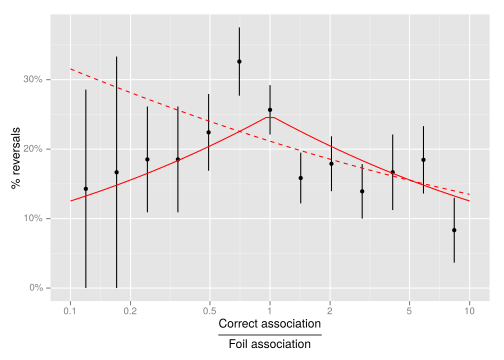
\includegraphics[width=.7\textwidth]{imgs/exp4_reversals.pdf}
  \caption[Proportion of correct responses that involved reversals,
  Experiment 4.]{
    The proportion of correct responses
    where participants initially moved towards the foil species.
    A model using the log-transformed association ratio as a predictor
    (dashed red line) showed that participants were more likely
    to produce these reversal trajectories when the association ratio
    favoured the foil species.
    However, the data were slightly better fit by a model (solid red line)
    which showed that these reversals were most likely to occur
    when the association ratio favoured neither response.
    \label{fig:exp4_reversals}
  }
\end{figure}

\begin{figure}[bp]
  \centering
  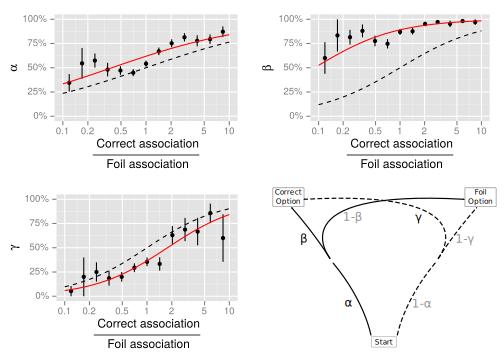
\includegraphics[width=.7\textwidth]{imgs/exp4_transitions_combined.pdf}
  \caption[Transition probabilities, as a function of the association ratio,
    in Experiment 4.]{
    \label{fig:exp4_transitions}
    Transitions probabilities from Experiment 4,
    as functions of the association ratios.
    As the association ratio increased in favour of the correct species,
    participants became more likely to initially move towards that species ($\alpha$, top left),
    to select that species after initially moving towards it ($\beta$, top right),
    and to select it even after initially moving towards the foil ($\gamma$, bottom left).
    Dashed lines show the expected values if participants were
    influenced by association ratio only.
    Overview of the three parameters can be seen in the bottom right.
  }
\end{figure}


The model for $\alpha$ (Figure~\ref{fig:exp4_transitions}, top left)
had a marginally significant positive intercept
($logit(\beta)$ = 62\%, CI = [50\%, 73\%], z = 1.886, p = .0593)
indicating that participants initially moved towards the correct species
on 62\% of trials when the ratio was $\frac{1}{1}$,
more than the 50\% that would be expected 
based on the association ratio alone.
The association ratio was also a significant positive predictor
($e^{\beta}$ = 1.7, CI = [1.4, 2.0], z = 6.109, p < .0001)
such that participants became more likely to initially move
towards the correct species as it was increasingly favoured by the association ratio.

The model for $\beta$  (Figure~\ref{fig:exp4_transitions}, top right)
had a robust positive intercept
($logit(\beta)$ = 80\%, CI = [85\%, 92\%], z = 10.567, p < .0001),
meaning that after initially moving towards the correct species,
participants selected that species 80\% of the time
when the association ratio was $\frac{1}{1}$.
The association ratio was also a significant positive predictor here
($e^{\beta}$ = 2.4, CI = [1.8, 3.2], z = 5.678, p < .0001),
meaning that participants became more likely to select the correct species
on trials where they initially moved towards it
as the association ratio in favour of the correct species increased.
In general, however, participants very rarely
changed direction after moving towards the correct species
in any case.

Finally, the model for $\gamma$  (Figure~\ref{fig:exp4_transitions}, bottom left)
contained a significant \emph{negative} intercept
($logit(\beta)$ = 37\%, CI = [30\%, 43\%], z = 3.963, p < .0001),
indicating that on trials where they initially moved towards the foil species,
participants only changed direction to select the correct species instead
37\% of the time when the association ratio was $\frac{1}{1}$.
The association ratio was again a positive predictor here
($e^{\beta}$ = 2.6, CI = [2.0, 3.5], z = 6.374, p < .0001),
meaning that as the strength of the association ratio
in favour of the correct species increased,
participants were more likely to switch direction
and select the correct species when they initially moved towards the foil.


\subsubsection{Time course}
\FloatBarrier

\begin{figure}[ht]
  \centering
  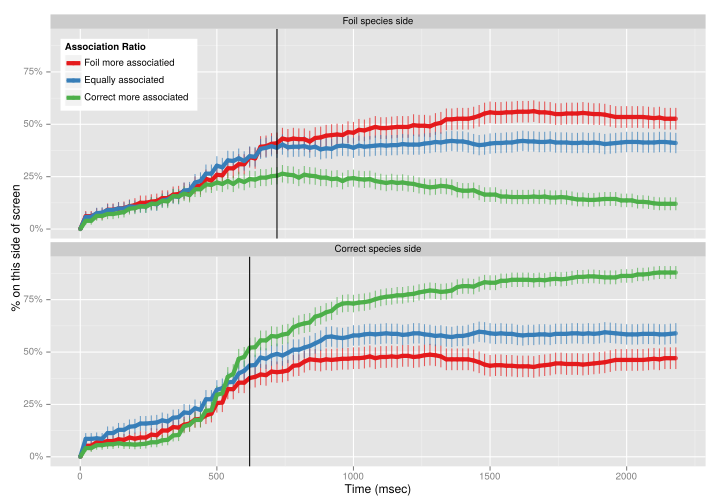
\includegraphics[width=\figurewidth]{imgs/exp4_condition_timecourse.pdf}
  \caption[Time course, separately for each response option, in Experiment 4.]{
    Proportion of trials on side of screen corresponding to the correct species (top)
    and the foil species (bottom) over time.
    The association ratio is a significant predictor
    of movements towards the foil from 720 msec,
    and of movements towards the correct species from 620 msec (solid vertical lines).
    \label{fig:exp4_condition_timecourse} }
\end{figure}


As usual, the time course of  the mouse movements here
reveals more about the points at which participants were
drawn towards each response.
Figure~\ref{fig:exp4_condition_timecourse} shows the proportion of trials
on the side of the screen corresponding to each species over time,
for trials where the association ratio favours the foil species (N = 359),
the two species were rated as equally associated (N = 397),
or the correct species was more strongly associated (N = 432).
To estimate divergence times,
I fitted two series of logistic mixed models,
one series predicting the probability of being on the foil species' side of the screen,
and one the probability of being on the correct species' side,
separately for every 20 msec time window.
Each model included the log-transformed association ratio  as a predictor,
and included random intercepts for each participant and each base species.
The divergence points were the times in each series
after which the association ratio is found to be a significant predictor.
The association ratio had a significant effect on
participants' probability of being on the foil species'
side of the screen from 720 msec,
and their probability of being on the correct species' side from 620 msec.

\begin{figure}[h]
  \centering
  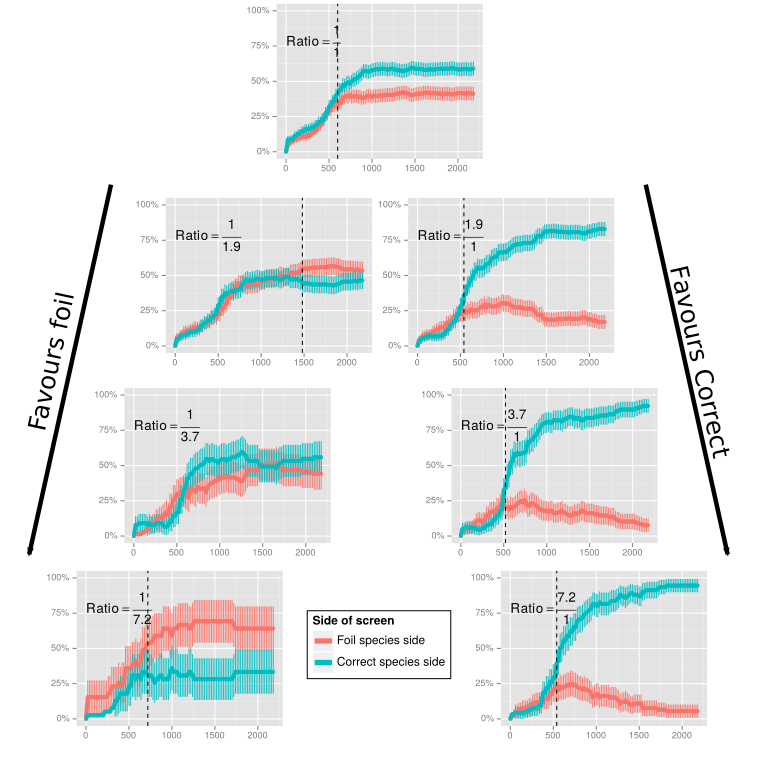
\includegraphics[width=\figurewidth]{imgs/exp4_ratio_timecourse.pdf}
  \caption[Time course, separately for different association ratios, in Experiment 4.]{
    Proportion of trials on the side of the screen corresponding to each response,
    grouped by association ratios.
    When the association ratio favours the correct option,
    %% \aside{This figure should have the divergence points marked for each trial,
    %%   a legend somewhere, and the font sizes all the same.
    %%   I will do this in the next few days when I've the use of a computer with a mouse.}
    \label{fig:exp4_ratio_timecourse} }
\end{figure}

\begin{table}
  \centering
  \caption[Divergence times, Experiment 4.]{
    Divergence times, and number of trials included,
    for each binned value of the association ratio.
    For ratios of $\frac{1}{7.2}$ and $\frac{1}{1.9}$,
    participants were significantly more likely to be on
    the foil species' side of the screen than the correct species'
    from the divergence time onwards.
    For all other ratios, participants were more likely to be on
    the correct species' side of the screen
    from the divergence time.
    \label{tab:exp4_ratio_timecourse_table}
  }
  \doublespacing
  \begin{tabular}{lrr}
    \toprule
    Ratio           & Divergence (msec) & N\\
    \midrule
    $\frac{1}{7.2}$ & 720               & 39\\
    $\frac{1}{3.7}$ & N/A               & 77\\
    $\frac{1}{1.9}$ & 1,480              & 243\\
    $\frac{1}{1}$   & 600               & 397\\
    $\frac{1.9}{1}$ & 540               & 223\\
    $\frac{3.7}{1}$ & 520               & 117\\
    $\frac{7.2}{1}$ & 540               & 92\\
    \bottomrule
  \end{tabular}
\end{table}

Figure~\ref{fig:exp4_ratio_timecourse}
shows the proportion of trials on either side of the screen,
with separate plots representing different levels of the association ratio.
For this analysis, I divided the log-transformed association ratio
into seven bins of equal width,
and labelled each bin according to the mean association ratio within it:
$\frac{1}{7.2}$, $\frac{1}{3.7}$, $\frac{1}{1.9}$, $\frac{1}{1}$, $  \frac{1.9}{1}$, $\frac{3.7}{1}$, and $\frac{7.2}{1}$.
Within each of these bins, I found the divergence point,
after which participants were more likely to be
on one side of the screen than the other,
by fitting a series of logistic mixed models,
comparing the probability of being on either side of the screen,
with random intercepts for each participant and each base species.

As the association ratio in favour of the correct species increased,
from $\frac{1}{1}$ (both species equally associated) up to $\frac{7.2}{1}$
(correct species 7.2 times more strongly associated than the foil),
we see a clear increase in the number of trials where
the cursor ends up on the correct species' side,
mirroring the earlier analysis of participants' responses.
There was little difference, however,
in the trends leading up to these final proportions.
For all of these bins, the preference for the correct species
emerged from 520 -- 600 msec,
and the shape of the curves were broadly similar,
except for the differences in their overall heights.
Thus, structured knowledge began to influence
participants' motor output from \tildetext600 msec.

When the association ratio was less than $\frac{1}{1}$, however,
and so conflicted with structured knowledge,
the trends were less clear.
When the ratio was strongest in favour of the foil species ($\frac{1}{7.2}$),
participants were more likely to move towards the foil
than the correct species from 720 msec.
Both species were equally attractive with a ratio $\frac{1}{3.7}$, however,
and with a ratio of $\frac{1}{1.9}$ a significant preference for the foil
only emerged from 1,480 msec.
Note, however, that even when the association ratio
conflicts with structured knowledge,
there is no evidence of a cross-over relationship ---
in each subplot within Figure~\ref{fig:exp4_ratio_timecourse},
participants were either drawn to the correct species, or to the foil,
but in no case were they primarily initially drawn towards the foil,
and later drawn towards the correct species.




\section{Discussion}

In this experiment, I combined mouse tracking with
a forced choice version of the base rate neglect task,
where I manipulated both the descriptions,
and the base rates participants reasoned about.
In doing so, I build on two lines of research.
Much earlier work in the heuristics and biases and dual process literature 
\citep[i.e.][]{Kahneman2011,Kahneman1973}
claims that descriptions are processed easily and automatically by Type 1 processes,
while processing base rate information
requires the optional later engagement
of more effortful Type 2 processes.
As a result, base rates are more likely to be ignored or underweighted.
More recent accounts \citep[i.e.][]{DeNeys2012,Barbey2007}
mostly agree with this fundamental dual process interpretation,
but argue that base rates play a more involved role in reasoning,
either because they can be processed by Type 1 processes 
\citep{DeNeys2012}, 
or because Type 1 and 2 processes operate in parallel
\citep{Sloman1996,Barbey2007}.


Analysis of problems in this experiment where
base rates and descriptions conflicted
provided support for a generic dual process account.
Participants gave the response cued by the description
on 80\% of such trials,
and when doing so were faster to read the description,
faster to respond,
and less likely to initially move the mouse cursor
towards the opposite option than on trials
where they gave the base rate-cued response.
Participants were also much more likely to
initially move the mouse cursor towards the description-cued option
than the base rate-cued option when the cues disagreed (doing so 66\% of the time),
and more likely to change direction if their initial movement
was towards the base rate-cued option.

Most dual processes accounts ---
the exception being a selective model \citep{Klaczynski2000,Chaiken1987}
where one or other kind of processing is engaged for a given task ---
would predict that participants who do give the response cued by the base rate
should be conflicted while doing so,
as they must inhibit the pull of the description-cued response.
This prediction was tested by analysing
all trials where participants could rely on the base rate,
and looking at effect of manipulating the description.

Consistent with this prediction,
the contents of a problem's description had a strong effect
on participants' base rate-cued reasoning,
as participants were most likely to give the base rate-cued response
when this response was also supported by the description (94\% of trials),
less likely when the description was uninformative (69\%),
and as mentioned above, only selected the base rate-cued response
when it conflicted with the description on 20\% of trials.

Similarly, when they did give this base rate-cued response,
participants both spent longer reading the description,
and spent longer responding,
when the description conflicted with the description than when it agreed.
This suggests that
participants had to inhibit the description-cued response
before they could give the base rate-cued response instead.
Unlike previous experiments in this thesis, however,
participants' were not significantly more likely to trace
reversal trajectories towards the base rate-cued option
under conflict, although the trend was in this direction.

The transition probability analysis (Table~\ref{tab:exp5_br_transitions})
similarly showed that descriptions had a pervasive effect
on participants' base rate-driven reasoning,
influencing both their initial movements,
and their ultimate responses regardless of initial movement direction.
The transition probabilities also allow us to
make sense of the non-significant effect of descriptions
on the probability of participants following a reversal trajectory
when giving the base rate-cued response.
Regardless of the base rate,
participants initially moved towards the description-cued option,
where available, on two thirds of trials.
Given that they were no more likely to initially
move towards the alternative option
when the base rate cued it than when it did not,
we must assume that base rates play no role at this point.
Later in reasoning, the influence of the description is even greater, 
dictating 80\% of final responses when it conflicts with the base rate,
and 94\% both when it agreed and when the base rate was uninformative.
At this point, base rates also clearly play a role,
as the response not cued by the description
is given on only 6\% of trials when it is not cued by the base rate either,
but 20\% when it is cued by the base rate.
To simplify, it appears that only the descriptions,
and random variations, have an effect on initial movements,
while later movements are even more influenced by descriptions,
and also slightly influenced by base rates.
The time course data are also in line with this interpretation,
as base rates had no influence on early movements.
When they did show an effect, after 740 msec,
this only slightly reduced the pull of the description-cued option
rather than reversing it,
as was the case in Experiments 1 and 2, for instance
(see the bottom panel of Figure~\ref{fig:exp5_timecourse}).





While these results are consistent with most
dual process accounts of this task,
some accounts, such as the intuitive logic theory \citep{DeNeys2012,Handley2015},
or a parallel-competitive dual process theory \citep{Barbey2007,Sloman1996},
further predict conflict in the opposite direction,
with participants who base their responses on descriptions
nevertheless showing sensitivity to the base rate information,
and experiencing conflict when base rates and descriptions disagree.

Analysis of participants' responses
on trials where the description cued a response showed
some evidence of sensitivity to base rates,
with participants less likely to give the description-cued response
when it conflicted with the base rate
than when the base rate agreed with the description, or was uninformative.
However, on such conflict trials participants
still overwhelmingly gave the response cued by the description.
Analysis of individual differences here
(Figure~\ref{fig:exp5_description_acc})
showed that the majority of participants' responses
appeared to be slightly influenced by the base rate,
with a small minority strongly influenced by it.

In contrast to previous tests of the intuitive logic theory, however,
\citep{DeNeys2008,DeNeys2008a,Franssens2009,Pennycook2012a}
there was no significant evidence that participants were
influenced by base rates on trials where their responses
were driven by the description,
as their reading times, movement initiation times,
response times, and cursor trajectories
did not differ significantly when the base rate
agreed with the description, was uninformative, or disagreed with it.
However, the trends were in the direction predicted by the intuitive logic account,
with participants slower to respond when the base rate conflicted with the description.
An exploratory Bayesian analysis suggested that
the most plausible effect size was a 2.8\% increase in response times under conflict,
although the data was largely inconclusive.
there was considerable uncertainty around this tiny effect.

Analyses of the transition probabilities
and the time course data told the same story.
Participants' initial mouse movements,
and the position of the cursor before 740 msec,
were not influenced by changes in the base rate
on trials where participants could rely on the description.
Instead, participants were slightly less likely
to select the description-cued response option,
or to be on its side of the screen from 740 msec onwards,
when the base rate cued the alternative response.
Taken together, these results suggest that
base rates either dictated participants' response to a problem,
or were almost totally ignored


To recapitulate, the results of this experiment
provide further support for a dual process interpretation
of base rate neglect \citep{Kahneman2002,Kahneman2005},
where, fast, effortless, automatic Type 1 processes
underlie description-based reasoning,
and slower, effortful Type 2 processes underlie
base rate-based reasoning.
Results consistent with this interpretation
were found in all of the analyses reported.
Participants predominantly gave the description-cued response
when the base rate also cued it and when the base rate was uninformative,
and only did so slightly less when the base rate conflicted with the base rate.
Even when giving base rate-cued responses,
participants were conflicted when the description disagreed with the base rate.
Analysis of the cursor trajectories and the time course data
showed that descriptions dictated both early movements (from half a second)
and participants' actual responses.

The data were less consistent, however, with some intuitive logic accounts
\citep[i.e.][]{DeNeys2012,DeNeys2014a,Handley2015}.
These would predict that
even when participants give the response cued by the description,
they should be sensitive to manipulations of the base rate,
and previous studies have found such effects
\citep[i.e.][]{DeNeys2008,Pennycook2012a,Pennycook2014}.
Here, I found no significant effects of manipulating the base rate
on participants' cursor movements or response times
when they gave the description-cued response.
An exploratory Bayesian analysis, however,
showed that participants were very slightly slower (around 30 msec)
on these trials when the base rate disagreed with the description.
Thus, it is not possible to draw strong conclusions
either for or against the intuitive logic account
from the current data.

The absence of a significant intuitive logic effect
on response times in particular was surprising,
as response times have been used as a measure of this conflict
in a number of previous studies \citep[i.e.][]{DeNeys2008,Pennycook2012a},
outlined in Table~\ref{tab:previous_baserate_studies}.
Although it is difficult to say with certainty
why this experiment differs from previous work,
I can identify a number of possibilities.

First, a number of changes were made to 
the procedure used by \citet{DeNeys2008a}
in order for it to be compatible with the mouse tracking paradigm.
As discussed above, the way in which information
was presented here meant that participants were able to
process each trials' information at two points:
before clicking on the ``NEXT'' button to reveal the question (reading time),
and after seeing the question but before responding (response time).
However, even when I combined these times (not reported),
there was little evidence of participants being slower
to give the description-cued response when it conflicted with the base rate.

The mouse tracking paradigm also requires that
participants respond under time pressure,
in this case within 6 seconds.
A visual timer in the centre of the screen
was used in this experiment to reinforce this idea,
filling up over the course of the allowed time.
As this time limit was only exceeded on 2 trials out of 2,000,
and average response times were below 2 seconds in all conditions,
I can be quite confident that participants did reason quickly,
although again this does not include
time spent reading the description.

These response are considerably faster than
those reported in the majority of previous conflict detection studies
that used the base rate paradigm
and measured response latencies, outlined in Table~\ref{tab:previous_baserate_studies}.
Moreover, of these studies, only two required participants to respond before a deadline.
\citet{DeNeys2008} presented participants in an fMRI scanner
with problems almost identical to those used here,
and required them to respond within 8.5 seconds of seeing the questions.
They found that participants were slower to give description-cued responses
when the cues conflicted (3.5 seconds) than any other condition ($\sim$2.8 seconds).
However, it should be noted that these response times were 
almost a second longer than those reported here,
at a time scale where this constitutes a $\sim$66\% increase.
Their result, while moderate in size ($\eta^2_p = .28$),
was also not robustly statistically significant,
with $F(1, 12) = 4.6, p_{rep} = .87$
(corresponding to approximately $p = .05$).

The other study reporting conflict effects at such a short time scale
was Experiment 2 of \citet{Pennycook2014},
where participants were asked to respond within 5 seconds.
Note, however, that this was an unusual base rate experiment.
Participants were instructed before each trial
to base their response on either ``belief'', or ``statistics'',
and in Experiment 2 asked to respond within 5 seconds.
Analysis of response latencies revealed conflict effects in both directions ---
when reasoning based on statistics, participants were slower 
if the description cued the opposite response,
and likewise slower when reasoning based on belief
if the base rate cued the opposite response.
However, these times remain a second or more slower
than those reported in the current experiment.
Furthermore, the magnitude of this effect was extremely small ---
going from 3.70 to 3.79 for statistics-based decisions ---
a small effect size ($\eta^2_p$) of .08.
It should also be noted that in Experiment 2 of \citet{Pennycook2014},
instructions to rely on belief or statistics were manipulated within-participants,
and so the effect within this short time window
could be in part due to task-switching effects \citep{Monsell2003}.
Experiment 3 of the same paper demonstrated
a similar effect with a between-participants manipulation,
but participants were not asked to respond quickly,
and the dependent variables were participants'
probability judgements and confidence ratings,
not their response times.
Therefore, it seems possible that in the current experiment
a) participants responded too quickly in most cases to detect 
the conflict between their responses and the base rate;
b) having not been explicitly told to use the base rate on 50\% of trials,
participants may have been less sensitive to the base rate
than those in  \citet{Pennycook2014}.

% \input{previous_baserate_studies_table}

\begin{table}
  \centering
  \caption[Prevous base rate neglect studies.]{
    Number of base rate-cued responses under conflict,
    and response latencies for description-cued responses
    when cues either agreed or conflicted,
    in previous base rate studies.}
  \label{tab:previous_baserate_studies}
  \rotatebox{90}{
    %% \begin{tabular}{ L{4cm} L{4cm} L{2cm} L{2cm} L{2cm}}
    \begin{tabular}{ p{.4\textwidth} p{.4\textwidth} p{.2\textwidth} p{.15\textwidth} p{.15\textwidth}}
      %% \begin{tabular}{\textwidth}{p{5cm}p{4cm}LLL}
      \toprule
      Study                                                                               &  Procedure                                          &  BR responses                &  No-conflict RT &  Conflict RT   \\[.75cm]
      \midrule                                         
      \citet{DeNeys2008a}                                                                 &  fMRI                                               &  45\%                        &  2.8            &  3.75          \\[.75cm]
      \citet{DeNeys2008}                                                                  &  Standard                                           &  22\%                        &  $\sim$14       &  $\sim$18      \\[.75cm]
      \citet{Franssens2009}                                                               &  Secondary load                                     &  47\%~(no~load) 35\%~(load ) &  $\sim$14       &  $\sim$17      \\[.75cm]
      \citeauthor{DeNeys2009a} (\citeyear{DeNeys2009a};~Exps.~2--4)                       &  Standard                                           &  $\sim$33\%                  &  $\sim$14       &  $\sim$17      \\[.75cm]
      %% \citet{DeNeys2011b}                                                              &  Confidence ratings                                 &  20\%                        &  NA             &  NA            \\[.75cm]
      \citeauthor{Pennycook2012a} (\citeyear{Pennycook2012a};~Exp.~4; extreme~base~rates) &  Standard                                           &  24--26\%                    &  16             &  20            \\[.75cm]
      \citeauthor{Pennycook2012b} (\citeyear{Pennycook2012b};~Initial responses)          &  Two-response paradigm \mbox{(probability~ratings)} &  N/A                         &  12.8           &  13.4          \\[.75cm]
      \citeauthor{Pennycook2014} (\citeyear{Pennycook2014};~Exp.~1)                       &  Belief/statistics instructions                     &  N/A                         &  $\sim$13       &  $\sim$14      \\[.75cm]
      \citeauthor{Pennycook2014} (\citeyear{Pennycook2014};~Exp.~2)                       &  Belief/statistics instructions, 5~second~deadline  &  N/A                         &  $\sim$3.8      &  $\sim$3.7     \\[.75cm]
      \bottomrule
    \end{tabular}
  }
  %% \end{tabulary}
\end{table}


Another factor may be the scarcity of base rate-cued responses
in general in the current experiment.
Reasonably, one would expect conflict detection to be 
related to participants' responses:
experiments that yield many base rate-cued responses
should also yield greater detection of conflict
on problems in which the description-cued response is given.
In this experiment, on the other hand,
the base rate-cued response was given on only 20\% of conflict problems,
perhaps unsurprisingly given the fast response times here,
and the robust finding that base rate responses
are slower than description responses.
Consequently, it may not be so surprising that
an experiment which yielded relatively few base rate-cued responses
should also show little influence of base rates 
on more subtle measures such as response time.

Lastly, recent work 
\citep[e.g.][]{DeNeys2010,Mevel2014} has highlighted
that there are individual differences in
this conflict detection process ---
not all participants are slower, or less confident,
when their responses conflict with base rates,
or with logical principles.
At present, we know relatively little about the factors
that make some participants, but not others,
sensitive to these conflicts.
Therefore, given that almost all studies in this area
reveal some participants for whom
the conflict detection effects do not hold,
it should perhaps not be surprising that 
these effects are not found in every study.

\subsubsection{Conclusions}

To conclude, this chapter reports one of the first uses of
the mouse tracking paradigm to investigate the interaction of
dual processes during reasoning.
Results are consistent with a default-interventionist
dual process accounts \citep{Evans2006,Kahneman2002,Evans2013a},
by which descriptions are processed easily and automatically
by Type 1 processes,
but base rates, thought to require Type 2 processes to process.
play less of a role in reasoning on most trials.
In fact, when the base rates were attended to,
they tended to dictate participants' responses outright.
The rich, temporal dynamics of the data collected
using this paradigm reveal much more about the underlying processes,
for instance that only descriptions influence
the initial direction of participants' cursor movements,
and that the descriptions have a discernible effect on cursor movements
from around 500 msec, while the weaker effect of base rates
is not apparent until around 750 msec.

A number of recent studies have also shown evidence
of conflict in the opposite direction,
as base rates have some effect on participants
even when their responses appear to be dictated by descriptions alone.
The current data, however, did not support this idea,
although this may in part be due to the ways in which
the experimental paradigm had to be adapted
to suit the mouse tracking paradigm,
in particular, the extremely faster response times,
and unusual presentation of information.
Despite this, however, the current chapter demonstrates 
another point at which conflict can be found in reasoning,
when the right kind of data is collected.

% % % % % % % % % % % % % % % % %
% % % % % % % % % % % % % % % % %
% % % % % % % % % % % % % % % % %
% % % % % % % % % % % % % % % % %











\begin{appendices}
  %% \setcounter{secnumdepth}{0}
  \appendixpage
  \graphicspath{{./../Appendices/}}

  \chapter{CRT Reasoning Problems from Experiment 6}\label{appendix:exp6_stimuli}
  \begin{center}
  \singlespacing
  \begin{longtable}{llrrlrr}
    \caption[]{
      Stimuli used in Experiment 6.
      Items 1--3 were adapted from \citet{Frederick2005}.
      Items 4--8 were adapted from \citet{Primi2015}.
      \emph{Note.} Percentages in parentheses show the proportion of participants who gave each response.
    }\\
    \toprule
    & \multicolumn{3}{l}{Conflict} & \multicolumn{3}{l}{No-conflict} \\
    \midrule
    \endfirsthead
    \toprule
    & \multicolumn{3}{l}{Conflict} & \multicolumn{3}{l}{No-conflict} \\
    \midrule
    \endhead

    \bottomrule
    \endfoot

    \bottomrule\bottomrule
    \endlastfoot

    1 &
    \multicolumn{3}{ p{.4\textwidth} }{
      A bat and a ball together costs £1.10.
      A bat costs £1 more than a ball.
      How~much~does~a~ball~cost?}
    & \multicolumn{3}{ p{.4\textwidth} }{
      A bat and a ball together costs £1.05.
      A bat costs £1.
      How much does a ball cost?
    } \\*
    \\*
    & Correct response:   & 5p   &(15\%) &  Correct response:  & 5p & (97\%)\\*
    & Heuristic response: & 10p   &(83\%) &  Foil response:     & 10p & (0\%)\\*
    & Foil response:      & 15p   &(0\%)  &  Foil response:    & 15p & (1\%)\\*
    & Foil response:      & 90p   &(2\%)  &  Foil response:    & 90p & (1\%)\\
    \midrule

    2 &
    \multicolumn{3}{ p{.4\textwidth} }{
      It takes 5 machines 5 minutes to make 5 
      widgets. How many minutes would it take 100
      machines to make 100 widgets?}
    & \multicolumn{3}{ p{.4\textwidth} }{
      It takes a machine 5 minutes to make 5 
      widgets. How many minutes would it take the
      machines to make 100 widgets?
    } \\*
    \\*
    & Correct response:   & 5   &(24\%) &  Correct response:  & 100 & (83\%)\\*
    & Heuristic response: & 100   &(69\%) &  Foil response:     & 5 & (2\%)\\*
    & Foil response:      & 50   &(4\%)  &  Foil response:    & 50 & (13\%)\\*
    & Foil response:      & 10   &(3\%)  &  Foil response:    & 10 & (2\%)\\
    \midrule

    3 &
    \multicolumn{3}{ p{.4\textwidth} }{
      In a lake, there is a patch of lily pads.
      Every day, the patch doubles in size.
      If it takes 48 days for the patch to cover
      the entire lake, how many days would it take
      for the patch to cover half of the lake?}
    & \multicolumn{3}{ p{.4\textwidth} }{
      In a lake, there is a patch of lily pads.
      Every day, the patch grows by 10m².
      If it takes 48 days for the patch to cover
      the 150m², how many days would it take
      for the patch to cover 140m²?
    } \\*
    \\*
    & Correct response:   & 47   &(25\%) &  Correct response:  & 47 & (79\%)\\*
    & Heuristic response: & 24   &(59\%) &  Foil response:     & 24 & (17\%)\\*
    & Foil response:      & 12   &(15\%)  &  Foil response:    & 12 & (4\%)\\*
    & Foil response:      & 2   &(2\%)  &  Foil response:    & 2 & (0\%)\\
    \bottomrule

    4 &
    \multicolumn{3}{ p{.4\textwidth} }{
      If you flipped a fair coin twice, what is
      the probability that it would land
      'Heads' at least once?}
    & \multicolumn{3}{ p{.4\textwidth} }{
      If you flipped a fair coin twice, what is
      the probability that it would land
      'Heads' exactly once?
    } \\*
    \\*
    & Correct response:   & 75\%   &(4\%) &  Correct response:  & 25\% & (68\%)\\*
    & Heuristic response: & 50\%   &(84\%) &  Foil response:     & 50\% & (26\%)\\*
    & Foil response:      & 25\%   &(11\%)  &  Foil response:    & 75\% & (6\%)\\*
    & Foil response:      & 100\%   &(1\%)  &  Foil response:    & 100\% & (0\%)\\
    \midrule

    5 &
    \multicolumn{3}{ p{.4\textwidth} }{
      If 3 elves can wrap 3 toys in
      1 hour, how many elves are needed
      to wrap 6 toys in 2 hours?}
    & \multicolumn{3}{ p{.4\textwidth} }{
      If 3 elves can wrap 3 toys in
      1 hour, how many toys could 6 elves
      wrap in half an hour?
    } \\*
    \\*
    & Correct response:   & 3   &(73\%) &  Correct response:  & 3 & (71\%)\\*
    & Heuristic response: & 6   &(22\%) &  Foil response:     & 6 & (20\%)\\*
    & Foil response:      & 1   &(2\%)  &  Foil response:    & 1 & (1\%)\\*
    & Foil response:      & 12   &(4\%)  &  Foil response:    & 12 & (8\%)\\*
    \midrule

    6 &
    \multicolumn{3}{ p{.4\textwidth} }{
      Ellen and Kim are running around a track.
      They run equally fast but Ellen started later.
      When Ellen has run 5 laps, Kim has run 10 laps.
      When Ellen has run 10 laps, how many has Kim run?}
    & \multicolumn{3}{ p{.4\textwidth} }{
      Ellen and Kim are running around a track.
      They started at the same time,
      but Kim is twice as fast as Ellen.
      When Ellen has run 5 laps, Kim has run 10 laps.
      When Ellen has run 10 laps, how many has Kim run?
    } \\*
    \\*
    & Correct response:   & 15   &(73\%) &  Correct response:  & 20 & (98\%)\\*
    & Heuristic response: & 20   &(27\%) &  Foil response:     & 15 & (2\%)\\*
    & Foil response:      & 5   &(0\%)  &  Foil response:    & 5 & (0\%)\\*
    & Foil response:      & 19   &(0\%)  &  Foil response:    & 19 & (0\%)\\
    \midrule

    7 &
    \multicolumn{3}{ p{.4\textwidth} }{
      Jerry received both the 15th highest and
      the 15th lowest mark in the class. How many
      students are there in the class?}
    & \multicolumn{3}{ p{.4\textwidth} }{
      Jerry received both the 2nd highest and
      the 2nd lowest mark in the class. How many
      students are there in the class?
    } \\*
    \\*
    & Correct response:   & 29   &(26\%) &  Correct response:  & 3 & (79\%)\\*
    & Heuristic response: & 30   &(72\%) &  Foil response:     & 2 & (13\%)\\*
    & Foil response:      & 40   &(2\%)  &  Foil response:    & 5 & (8\%)\\*
    & Foil response:      & 5   &(0\%)  &  Foil response:    & 10 & (0\%)\\
    \midrule

    8 &
    \multicolumn{3}{ p{.4\textwidth} }{
      In an athletics team tall members tend to win
      three times as many medals than short members.
      This year the team has won 60 medals so far.
      How many of these have been won by short athletes?}
    & \multicolumn{3}{ p{.4\textwidth} }{
      In an athletics team tall members tend to win
      twice as many medals than short members.
      This year the team has won 60 medals so far.
      How many of these have been won by short athletes?
    } \\*
    \\*
    & Correct response:   & 15   &(44\%) &  Correct response:  & 20 & (58\%)\\*
    & Heuristic response: & 20   &(52\%) &  Foil response:     & 15 & (12\%)\\*
    & Foil response:      & 30   &(1\%)  &  Foil response:    & 30 & (27\%)\\*
    & Foil response:      & 50   &(3\%)  &  Foil response:    & 50 & (4\%)\\
  \end{longtable}
\end{center}

%% \begin{table}[!h]
%%   \centering
%%   \caption[]{
%%     Stimuli used in Experiment 6.
%%     Items 1--3 were adapted from \citet{Frederick2005}.
%%     Items 4--8 were adapted from \citet{Primi2015}.
%%     \emph{Note.} Percentages in parentheses show the proportion of participants who gave each response.
%%   }
%%   \singlespacing
%%   \footnotesize
%%   \begin{tabular}{llrrlrr}
%%     \toprule
%%     & \multicolumn{3}{l}{Conflict} & \multicolumn{3}{l}{No-conflict} \\
%%     \midrule

%%     %% \parbox[b]{2mm}{\multirow{6}{*}{\rotatebox[origin=c]{90}{1. Bat-and-ball}}} &
%%     1 &
%%     \multicolumn{3}{ p{.4\textwidth} }{
%%       A bat and a ball together costs £1.10.
%%       A bat costs £1 more than a ball.
%%       How~much~does~a~ball~cost?}
%%     & \multicolumn{3}{ p{.4\textwidth} }{
%%       A bat and a ball together costs £1.05.
%%       A bat costs £1.
%%       How much does a ball cost?
%%     } \\
%%     \\
%%     & Correct response:   & 5p   &(15\%) &  Correct response:  & 5p & (97\%)\\*
%%     & Heuristic response: & 10p   &(83\%) &  Foil response:     & 10p & (0\%)\\*
%%     & Foil response:      & 15p   &(0\%)  &  Foil response:    & 15p & (1\%)\\*
%%     & Foil response:      & 90p   &(2\%)  &  Foil response:    & 90p & (1\%)\\*
%%     \midrule

%%     2 &
%%     \multicolumn{3}{ p{.4\textwidth} }{
%%       It takes 5 machines 5 minutes to make 5 
%%       widgets. How many minutes would it take 100
%%       machines to make 100 widgets?}
%%     & \multicolumn{3}{ p{.4\textwidth} }{
%%       It takes a machine 5 minutes to make 5 
%%       widgets. How many minutes would it take the
%%       machines to make 100 widgets?
%%     } \\
%%     \\
%%     & Correct response:   & 5   &(24\%) &  Correct response:  & 100 & (83\%)\\*
%%     & Heuristic response: & 100   &(69\%) &  Foil response:     & 5 & (2\%)\\*
%%     & Foil response:      & 50   &(4\%)  &  Foil response:    & 50 & (13\%)\\*
%%     & Foil response:      & 10   &(3\%)  &  Foil response:    & 10 & (2\%)\\*
%%     \midrule

%%     3 &
%%     \multicolumn{3}{ p{.4\textwidth} }{
%%       In a lake, there is a patch of lily pads.
%%       Every day, the patch doubles in size.
%%       If it takes 48 days for the patch to cover
%%       the entire lake, how many days would it take
%%       for the patch to cover half of the lake?}
%%     & \multicolumn{3}{ p{.4\textwidth} }{
%%       In a lake, there is a patch of lily pads.
%%       Every day, the patch grows by 10m².
%%       If it takes 48 days for the patch to cover
%%       the 150m², how many days would it take
%%       for the patch to cover 140m²?
%%     } \\
%%     \\
%%     & Correct response:   & 47   &(25\%) &  Correct response:  & 47 & (79\%)\\*
%%     & Heuristic response: & 24   &(59\%) &  Foil response:     & 24 & (17\%)\\*
%%     & Foil response:      & 12   &(15\%)  &  Foil response:    & 12 & (4\%)\\*
%%     & Foil response:      & 2   &(2\%)  &  Foil response:    & 2 & (0\%)\\*
%%     \bottomrule
%%   \end{tabular}
%% \end{table}

%% \begin{table}
%%   \centering
%%   \footnotesize
%%   \begin{tabular}{llrrlrr}
%%     \toprule
%%     & \multicolumn{3}{l}{Conflict} & \multicolumn{3}{l}{No-conflict} \\
%%     \midrule

%%     4 &
%%     \multicolumn{3}{ p{.4\textwidth} }{
%%       If you flipped a fair coin twice, what is
%%       the probability that it would land
%%       'Heads' at least once?}
%%     & \multicolumn{3}{ p{.4\textwidth} }{
%%       If you flipped a fair coin twice, what is
%%       the probability that it would land
%%       'Heads' exactly once?
%%     } \\
%%     \\
%%     & Correct response:   & 75\%   &(4\%) &  Correct response:  & 25\% & (68\%)\\*
%%     & Heuristic response: & 50\%   &(84\%) &  Foil response:     & 50\% & (26\%)\\*
%%     & Foil response:      & 25\%   &(11\%)  &  Foil response:    & 75\% & (6\%)\\*
%%     & Foil response:      & 100\%   &(1\%)  &  Foil response:    & 100\% & (0\%)\\*    
%%     \midrule

%%     5 &
%%     \multicolumn{3}{ p{.4\textwidth} }{
%%       If 3 elves can wrap 3 toys in
%%       1 hour, how many elves are needed
%%       to wrap 6 toys in 2 hours?}
%%     & \multicolumn{3}{ p{.4\textwidth} }{
%%       If 3 elves can wrap 3 toys in
%%       1 hour, how many toys could 6 elves
%%       wrap in half an hour?
%%     } \\
%%     \\
%%     & Correct response:   & 3   &(73\%) &  Correct response:  & 3 & (71\%)\\*
%%     & Heuristic response: & 6   &(22\%) &  Foil response:     & 6 & (20\%)\\*
%%     & Foil response:      & 1   &(2\%)  &  Foil response:    & 1 & (1\%)\\*
%%     & Foil response:      & 12   &(4\%)  &  Foil response:    & 12 & (8\%)\\*
%%     \midrule

%%     6 &
%%     \multicolumn{3}{ p{.4\textwidth} }{
%%       Ellen and Kim are running around a track.
%%       They run equally fast but Ellen started later.
%%       When Ellen has run 5 laps, Kim has run 10 laps.
%%       When Ellen has run 10 laps, how many has Kim run?}
%%     & \multicolumn{3}{ p{.4\textwidth} }{
%%       Ellen and Kim are running around a track.
%%       They started at the same time,
%%       but Kim is twice as fast as Ellen.
%%       When Ellen has run 5 laps, Kim has run 10 laps.
%%       When Ellen has run 10 laps, how many has Kim run?
%%     } \\
%%     \\
%%     & Correct response:   & 15   &(73\%) &  Correct response:  & 20 & (98\%)\\*
%%     & Heuristic response: & 20   &(27\%) &  Foil response:     & 15 & (2\%)\\*
%%     & Foil response:      & 5   &(0\%)  &  Foil response:    & 5 & (0\%)\\*
%%     & Foil response:      & 19   &(0\%)  &  Foil response:    & 19 & (0\%)\\*
%%     \midrule

%%     7 &
%%     \multicolumn{3}{ p{.4\textwidth} }{
%%       Jerry received both the 15th highest and
%%       the 15th lowest mark in the class. How many
%%       students are there in the class?}
%%     & \multicolumn{3}{ p{.4\textwidth} }{
%%       Jerry received both the 2nd highest and
%%       the 2nd lowest mark in the class. How many
%%       students are there in the class?
%%     } \\
%%     \\
%%     & Correct response:   & 29   &(26\%) &  Correct response:  & 3 & (79\%)\\*
%%     & Heuristic response: & 30   &(72\%) &  Foil response:     & 2 & (13\%)\\*
%%     & Foil response:      & 40   &(2\%)  &  Foil response:    & 5 & (8\%)\\*
%%     & Foil response:      & 5   &(0\%)  &  Foil response:    & 10 & (0\%)\\*
%%     \midrule

%%     8 &
%%     \multicolumn{3}{ p{.4\textwidth} }{
%%       In an athletics team tall members tend to win
%%       three times as many medals than short members.
%%       This year the team has won 60 medals so far.
%%       How many of these have been won by short athletes?}
%%     & \multicolumn{3}{ p{.4\textwidth} }{
%%       In an athletics team tall members tend to win
%%       twice as many medals than short members.
%%       This year the team has won 60 medals so far.
%%       How many of these have been won by short athletes?
%%     } \\
%%     \\
%%     & Correct response:   & 15   &(44\%) &  Correct response:  & 20 & (58\%)\\*
%%     & Heuristic response: & 20   &(52\%) &  Foil response:     & 15 & (12\%)\\*
%%     & Foil response:      & 30   &(1\%)  &  Foil response:    & 30 & (27\%)\\*
%%     & Foil response:      & 50   &(3\%)  &  Foil response:    & 50 & (4\%)\\*

%%     \bottomrule
%%   \end{tabular}
%% \end{table}



  \chapter{Individual differences in Experiment 6 time course analyses}
  \label{appendix:exp6_participants}
  
Following previous intuitive logic studies \citep[e.g.][]{Mevel2014}
I calculated the number of heuristic responses given
by each participant on conflict problems, 
and categorised each participant as either
``majority heuristic'' (3 or 4 heuristic responses out of four, 53 participants)
or ``minority heuristic'' (0 to 2 heuristic responses, 75 participants).
In this appendix, I repeat the time course analyses
reported for Experiment 6 separately for each group of participants.
As none of the trends differ qualitatively from the results
reported in Chapter 6 in ways that affect my conclusions,
I do not provide interpretation of each individual figure.


\begin{figure}[h]
  \centering
  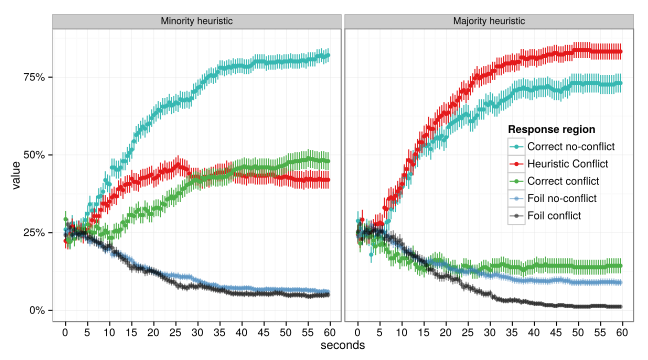
\includegraphics[width=.9\textwidth]{imgs/exp6/all_bias.pdf}
  %% \caption[Proportion of mouse cursors in each responses' region of the screen over time,
  %%   for minority heuristic and majority heuristic particiapants, 
  %%   Experiment 6.]{
  \caption[]{
    Proportion of mouse cursors in the region of the screen 
    corresponding to each response options, over time, 
    for conflict and no-conflict problems,
    separately for minority heuristic and majority heuristic participants
    (see also Figure~\ref{fig:exp6-all}).
  }
\end{figure}

\begin{figure}[h]
  \centering
  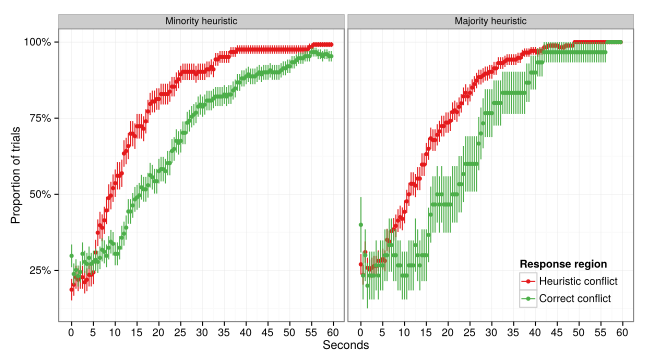
\includegraphics[width=.9\textwidth]{imgs/exp6/conflict-to-chosen_bias.pdf}
  %% \caption[Proportion of cursor in region of chosen response option
  %%   for minority heuristic and majority heuristic particiapants, 
  %%   Experiment 6.]{
  \caption[]{
    Proportion of mouse cursors in the region of
    the response option which was ultimately selected on that trial,
    comparing movements to the heuristic and correct options on conflict problems,
    separately for minority heuristic and majority heuristic participants
    (see also Figure~\ref{fig:exp6-all-to-chosen}).
  }
\end{figure}

\begin{figure}[h]
  \centering
  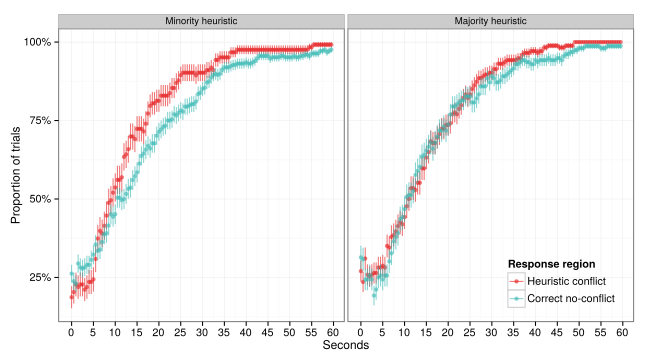
\includegraphics[width=.9\textwidth]{imgs/exp6/intuitive-to-chosen_bias.pdf}
  %% \caption[for minority heuristic and majority heuristic particiapants, 
  %%   Experiment 6.]{
  \caption[]{
    Proportion of mouse cursors in the region of
    the response option which was ultimately selected on that trial,
    comparing movements to the heuristic option conflict problems
    to those to the correct options on no-conflict problems,
    separately for minority heuristic and majority heuristic participants
    (see also Figure~\ref{fig:exp6-all-to-chosen}).
  }
\end{figure}

\begin{figure}[h]
  \centering
  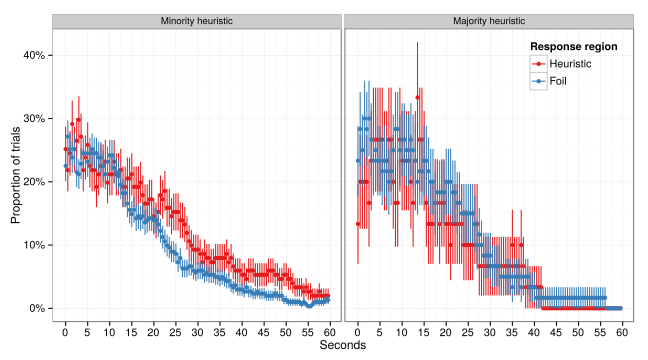
\includegraphics[width=.9\textwidth]{imgs/exp6/correct-not-chosen_bias.pdf}
  %% \caption[Proportion of cursor in region of other response options
  %%   when correct response was given
  %%   for minority heuristic and majority heuristic particiapants, 
  %%   Experiment 6.]{
  \caption[]{   
    Proportion of trials in the region of each option, over time,
    for trials in which the correct option was eventually chosen,
    separately for minority heuristic and majority heuristic participants
    (see also Figure~\ref{fig:exp6-correct-not-chosen}).
    Error bars show standard error of measurement.
  }
\end{figure}

\begin{figure}[h]
  \centering
  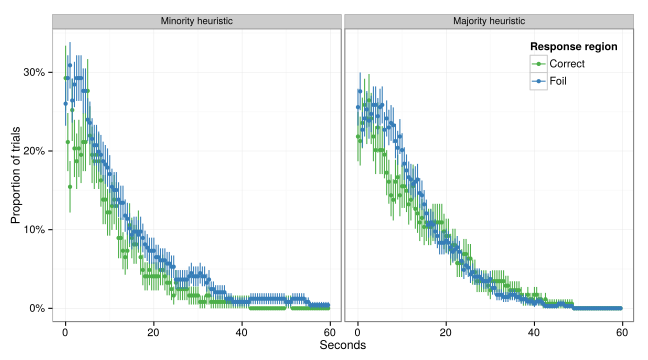
\includegraphics[width=.9\textwidth]{imgs/exp6/heuristic-not-chosen_bias}
  %% \caption[Proportion of cursor in region of other response options
  %%   when heuristic response was given,
  %%   for minority heuristic and majority heuristic particiapants, 
  %%   Experiment 6.]{
  \caption[]{
    Proportion of trials in the region of each option, over time,
    for trials in which the intuitive option was eventually chosen,
    separately for minority heuristic and majority heuristic participants
    (see also Figure~\ref{fig:exp6-heuristic-not-chosen}).
  }
\end{figure}


  \chapter{Differences between problems in Experiment 6 time course analyses}
  \label{appendix:exp6_items}
  
In this Appendix, I plot the time course analyses
for Experiment 6, reported in Chapter 6,
separately for each of the eight CRT problems.
The text of the conflict and no-conflict versions
of the eight items are shown in Appendix~\ref{appendix:exp6_stimuli}.

For clarity, I use labels to refer to each CRT problems.
Therefore, problems 1, 2, and 3 in Appendix~\ref{appendix:exp6_stimuli}
\citep[the original CRT items, from][]{Frederick2005} will be referred to as
the \emph{bat-and-ball}, \emph{widgets}, and \emph{lily pad} problems respectively.
Similarly, problems 5 -- 8, adapted from \citet{Primi2015},
will be referred to the
\emph{coin} (4),
\emph{elves} (5),
\emph{running track} (6),
\emph{grades} (7),
and \emph{athletics team} (8)
problems.


\begin{figure}[h]
  \centering
  \includegraphics[width=.9\textwidth]{imgs/exp6/all_items.pdf}
  %% \caption[Proportion of mouse cursors in each responses' region of the screen over time,
  %% seperately for each problem, Experiment 6.]{
  \caption[]{
    Proportion of mouse cursors in the region of the screen 
    corresponding to each response options, over time, 
    for conflict and no-conflict problems,
    separately for each CRT problem
    (see also Figure~\ref{fig:exp6-all}).
  }
\end{figure}

\begin{figure}[h]
  \centering
  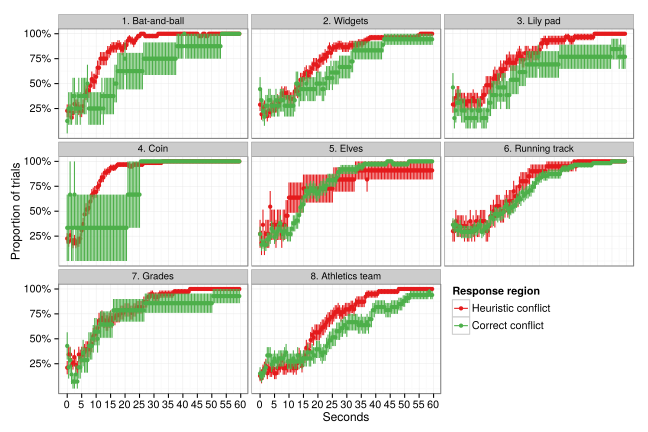
\includegraphics[width=.9\textwidth]{imgs/exp6/conflict-to-chosen_items.pdf}
  %% \caption[Proportion of cursors in region of chosen option,
  %% on conflict problems,
  %% seperately for each problem, Experiment 6.]{
  \caption[]{
    Proportion of mouse cursors in the region of
    the response option which was ultimately selected on that trial,
    comparing movements to the heuristic and correct options on conflict problems,
    separately for each CRT problem
    (see also Figure~\ref{fig:exp6-all-to-chosen}).
  }
\end{figure}

\begin{figure}[h]
  \centering
  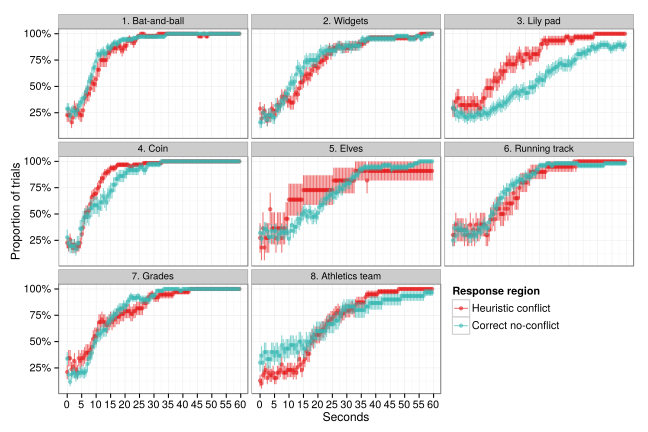
\includegraphics[width=.9\textwidth]{imgs/exp6/intuitive-to-chosen_items.pdf}
  %% \caption[Proportion of cursors in region of chosen option,
  %% for heuristically-cued responses,
  %% seperately for each problem, Experiment 6.]{
  \caption[]{
    Proportion of mouse cursors in the region of
    the response option which was ultimately selected on that trial,
    comparing movements to the heuristic option conflict problems
    to those to the correct options on no-conflict problems,
    separately for each CRT problem
    (see also Figure~\ref{fig:exp6-all-to-chosen}).
    \label{fig:exp6-heuristic-to-chosen-by-item}
  }
\end{figure}


\begin{figure}[h]
  \centering
  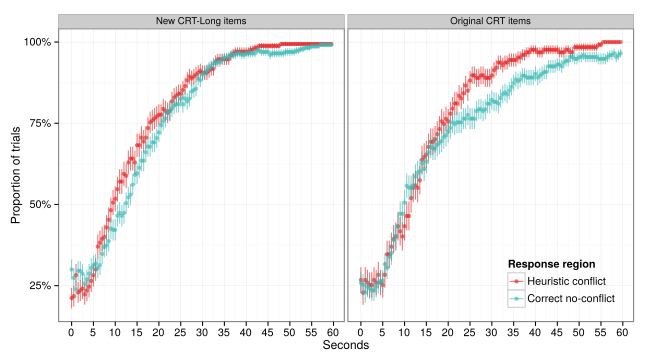
\includegraphics[width=.9\textwidth]{imgs/exp6/intuitive-to-chosen_oldnew.pdf}
  %% \caption[Proportion of cursors in region of chosen option,
  %% for heuristically-cued responses,
  %% seperately for original and extended CRT problems, Experiment 6.]{
  \caption[]{
    Proportion of mouse cursors in the region of
    the response option which was ultimately selected on that trial,
    comparing movements to the heuristic option conflict problems
    to those to the correct options on no-conflict problems,
    separately for the original problems adapted from \citet{Frederick2005},
    and the problems adapted from \citet{Primi2015}
    (see also Figure~\ref{fig:exp6-all-to-chosen}).
  }
\end{figure}




\begin{figure}[h]
  \centering
  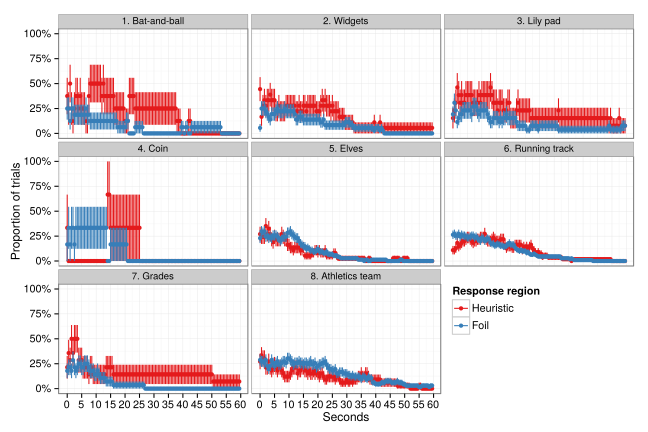
\includegraphics[width=.9\textwidth]{imgs/exp6/correct-not-chosen_items.pdf}
  %% \caption[Proportion of cursor in region of other response options
  %%   when correct response was given,
  %%   seperately for each problem, Experiment 6.]{
  \caption[]{
    Proportion of trials in the region of each option, over time,
    for trials in which the correct option was eventually chosen,
    separately for each CRT problem
    (see also Figure~\ref{fig:exp6-correct-not-chosen}).
    Error bars show standard error of measurement.
  }
\end{figure}

\begin{figure}[h]
  \centering
  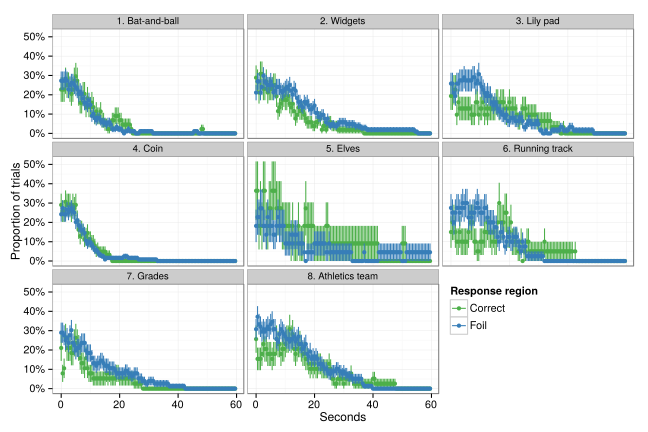
\includegraphics[width=.9\textwidth]{imgs/exp6/heuristic-not-chosen_items.pdf}
  %% \caption[Proportion of cursor in region of other response options
  %%   when heuristic response was given,
  %%   seperately for each problem, Experiment 6.]{
  \caption[]{
    Proportion of trials in the region of each option, over time,
    for trials in which the intuitive option was eventually chosen,
    separately for each CRT problem
    (see also Figure~\ref{fig:exp6-heuristic-not-chosen}).
  }
\end{figure}


\end{appendices}


\bibliography{../references}
\addcontentsline{toc}{chapter}{References}

\end{document}
